\documentclass[10pt,a4paper]{article}
\usepackage[T1]{fontenc}
\usepackage[utf8]{inputenc}
\usepackage{lmodern,microtype}
\renewcommand{\familydefault}{\sfdefault}
\usepackage[a4paper,left=22mm,right=22mm,top=22mm,bottom=21mm,headheight=14pt,headsep=7mm,footskip=10mm]{geometry}
\usepackage{amsmath,amssymb,amsthm,mathtools,bm}
\usepackage{graphicx,booktabs,tabularx,array,multirow,longtable}
\usepackage[table]{xcolor}
\usepackage{tikz}
\usetikzlibrary{arrows.meta,positioning,calc}
\usepackage[most]{tcolorbox}
\usepackage{enumitem,fancyhdr,lastpage,titlesec,caption,listings}
\usepackage{hyperref}
\hypersetup{colorlinks=true,linkcolor=teal!60!black,citecolor=teal!60!black,urlcolor=teal!60!black,
 pdftitle={WANTWOMBAN | Operator I - Sub-version 1.1},
 pdfauthor={Tom Klootwijk (supplied framework)},
 pdfsubject={Rim geometry, slit optics, strain transduction and verified physical feedback},
 pdfkeywords={WANTWOMBAN, Operator I, OTAN2, strain gauge, double verification, Klein seam, PSI}}
\definecolor{ink}{HTML}{173342}
\definecolor{accent}{HTML}{166C72}
\definecolor{light}{HTML}{EFF5F5}
\definecolor{muted}{HTML}{5B6C75}
\definecolor{line}{HTML}{CBD9DC}
\color{ink}
\setlength{\parindent}{0pt}
\setlength{\parskip}{6pt plus 1pt}
\linespread{1.10}
\setlength{\emergencystretch}{2em}
\titleformat{\section}{\Large\bfseries\color{ink}}{\thesection}{0.7em}{}
\titleformat{\subsection}{\normalsize\bfseries\color{accent}}{\thesubsection}{0.7em}{}
\titlespacing*{\section}{0pt}{0pt}{12pt}
\titlespacing*{\subsection}{0pt}{10pt}{3pt}
\setcounter{tocdepth}{1}
\numberwithin{equation}{section}
\newtheorem{proposition}{Proposition}[section]
\newtheorem{definition}{Definition}[section]
\newcolumntype{Y}{>{\raggedright\arraybackslash}X}
\newcolumntype{P}[1]{>{\raggedright\arraybackslash}p{#1}}
\renewcommand{\arraystretch}{1.25}
\captionsetup{font=small,labelfont=bf,skip=5pt}
\pagestyle{fancy}
\fancyhf{}
\fancyhead[L]{\scriptsize\bfseries WANTWOMBAN \enspace|\enspace OPERATOR I}
\fancyhead[R]{\scriptsize SUB-VERSION 1.1}
\fancyfoot[L]{\scriptsize\color{muted}Tom Klootwijk / supplied framework}
\fancyfoot[R]{\scriptsize\thepage\ /\ \pageref*{LastPage}}
\renewcommand{\headrulewidth}{0.4pt}
\newtcolorbox{keybox}[1][]{colback=light,colframe=line,boxrule=0.6pt,arc=0pt,left=9pt,right=9pt,top=7pt,bottom=7pt,title=#1,fonttitle=\bfseries,coltitle=ink,colbacktitle=light}
\newcommand{\src}[1]{\textcolor{muted}{\footnotesize Source basis: #1.}}
\newcommand{\newpart}{\clearpage}
\newcommand{\bb}{\{0,1\}}
\newcommand{\opI}{\mathcal{I}}
\newcommand{\R}{\mathbb{R}}
\newcommand{\ind}{\mathbf{1}}
\newcommand{\dd}{\,\mathrm{d}}
\DeclareMathOperator{\tr}{tr}
\DeclareMathOperator{\diag}{diag}
\DeclareMathOperator{\sgn}{sgn}
\DeclareMathOperator{\rank}{rank}
\DeclareMathOperator{\clip}{clip}
\DeclareMathOperator{\sym}{sym}
\lstset{basicstyle=\ttfamily\scriptsize,columns=fullflexible,keepspaces=true,breaklines=true,frame=single,rulecolor=\color{line},backgroundcolor=\color{light},showstringspaces=false}

\begin{document}
\thispagestyle{empty}
{\small\bfseries\color{accent}PHYSICAL FORMALIZATION / DEVELOPMENT EDITION}\hfill{\small 15 SEPTEMBER 2026}
\vspace*{27mm}

{\fontsize{35}{39}\selectfont\bfseries WANTWOMBAN}\par
\vspace{7mm}
{\fontsize{29}{34}\selectfont\color{accent}\textbar\ Operator I}\par
\vspace{9mm}
{\Large Rim geometry, slit optics, strain transduction\par
and verified physical feedback}\par
\vspace{7mm}
{\large Sub-version 1.1 of the WANTWOMBAN 1.0 formalization}

\vspace{15mm}
\noindent\textcolor{accent}{\rule{\linewidth}{0.8pt}}
\vspace{7mm}
{\small\color{muted}FRAMEWORK ATTRIBUTION / AS SUPPLIED}\par
{\Large\bfseries Tom Klootwijk}\par
{\normalsize NL200678942\quad /\quad 10-07-1990}

\vfill
\begin{keybox}[THE NEW FORMAL OBJECT]
A causal interaction-and-instrumentation operator that couples the existing 64-bit engine to a deformable rim, a specified optical aperture, calibrated strain and optical measurements, a material response, and a one-bit event decision.
\[
\text{word}\ \longrightarrow\ \text{geometry and actuation}\ \longrightarrow\ \text{physical interaction}
\]
\[
\text{physical interaction}\ \longrightarrow\ \text{two-channel evidence}\ \longrightarrow\ \text{verified event}\ \longrightarrow\ \text{word}
\]
\end{keybox}
\vspace{4mm}
{\small The parent formalization, both new source PDFs, the original Markdown, reference software, calculation results and a source manifest are embedded as attachments.}

\newpart
\section*{Document map}
\begingroup
\small
\setlength{\parskip}{0pt}
\makeatletter
\renewcommand{\l@section}[2]{\vskip .50em\@dottedtocline{1}{0em}{2em}{\bfseries #1}{#2}}
\@starttoc{toc}
\makeatother
\endgroup
\vfill
\begin{keybox}[HOW TO READ THIS SUB-VERSION]
\textbf{Source} identifies content actually present in the supplied documents. \textbf{Definition} fixes the new operator or protocol. \textbf{Physical model} supplies explicit assumptions and parameters. \textbf{Derived result} follows from those definitions or models. \textbf{Measured} is reserved for observations: no device measurements were supplied for this edition.

Source references use PDF page numbers counting the cover as page 1. The parent PDF's printed page numbers are one lower after its cover.
\end{keybox}

\newpart
\section{What improves in version 1.1}
\src{\textnormal{[S0]} WANTWOMBAN 1.0; \textnormal{[S1]} lily-pad transcript; \textnormal{[S2]} strain-gauge transcript; \textnormal{[S3]} originating Markdown}

The strongest development is to turn your proposed connection between \textbf{rim, pupil, material response and verification} into an instrument whose variables can be measured and whose decisions can be checked. Version 1.0 already supplies a corrected state engine and thermochromic feedback loop. This sub-version adds the missing mechanical and optical interfaces rather than replacing that architecture.

\begin{tabularx}{\linewidth}{@{}P{32mm}YY@{}}
\toprule
\textbf{Area} & \textbf{What the documents contribute} & \textbf{Formal improvement here}\\
\midrule
Rim and radial support & Upturned leaf rim, underside ribs and a large exposed surface [S1, pp.~1--3]. & A rim/rib domain, elastic deformation, specified supports and a stiffness--sensitivity trade-off.\\
Slit and liquid lens & A ``tilt-shifted rim,'' variable convexity and dichromatic sensing [S1, pp.~3--4]. & Separate aperture, refraction, diffraction, two spectral channels and absorbed power.\\
Strain-grid geometry & $R=\rho L/A$, Poisson contraction and foil-grid geometry [S2, pp.~1--3]. & Finite-deformation resistance, directional strain, weighted trace response and calibration.\\
Bridge readout & Exact divider equation and a quarter-bridge approximation [S2, p.~5]. & One declared polarity, its correct negative sign, exact inverse and thermal-bias accounting.\\
Double verification & A primary optical response and a second material-state witness [S1, pp.~5--7]. & A joint-event rule with timing, false-acceptance and missed-event probabilities.\\
Engine and feedback & OTAN2, pinion matrices, parity, Klein closure, PSI and thermochromic output [S0]. & An unchanged core word with typed sensor records and deformation-aware pruning.\\
\bottomrule
\end{tabularx}

\subsection*{The proposed meaning of Operator I}
The title requested here is \textbf{WANTWOMBAN | Operator I}. In this edition, $\opI$ is defined as the \textbf{interaction-and-instrumentation operator}. The vertical bar is the title separator and a visual reference to the slit. This is a new definition introduced for this sub-version; the source PDFs do not already specify a mathematical operator named $\opI$.

\subsection*{What remains intact}
The parent word layout, grouped OTAN2 profile, fixed-point Pinion Double Hadamard map, parity shifts, finite-depth seam rule, external thermal registers and distinction between occupancy and signed distance are retained. The original $\chi$ and cycle labels remain symbolic inputs; no new biological interpretation is attached to their bits. [S0, PDF pp.~5--12.]

\newpart
\section{Source-to-improvement change register}
\label{sec:register}
The new PDFs are saved conversations, containing your prompts and earlier generated explanations. The register below distinguishes an originating idea from a later explanation that overstates what the idea establishes. Original files are preserved unchanged.

\small
\begin{longtable}{@{}P{34mm}P{54mm}P{66mm}@{}}
\toprule
\textbf{Source location} & \textbf{Point requiring precision} & \textbf{Version 1.1 resolution}\\
\midrule
\endhead
{}[S1], pp.~2--3 & Rim is said to ensure flat radial growth and make a ``solar dish.'' & Structural support and optical concentration are different mechanisms. Use elastic compliance and intercepted power; do not identify an upturned rim with a focusing reflector.\\
{}[S1], pp.~1--3 & Fixed carrying capacity and complete exclusion of light beneath the leaf. & No load geometry, specimen dimensions, transmission spectrum or measurements accompany those numbers. Replace them with load/support and optical-transmission variables.\\
{}[S1], p.~4 & Slit edges are described as a waveguide; lensing allegedly increases photon speed and eliminates aberrations. & Aperture transmission, lens phase and propagation are separately specified. A static passive lens redistributes the field; it does not increase $h\nu$. Aberration and diffraction remain test quantities.\\
{}[S1], p.~4 & The panda example is assigned exact blue/green cone channels. & Retain a two-band engineering profile. The cited behavioral study supports color discrimination, not a measurement of two exact cone-response curves. [R4]\\
{}[S1], pp.~5--7 & Cellulose ``burning,'' two observations of one photon, and absolute zero false positives. & Preserve a material-state witness as a proposed engineered channel. Specify absorption, supplied energy, chemistry and noise; compute a joint detection probability.\\
{}[S1], p.~6 & Five to nine photons within a fixed interval are presented as a universal gate for seeing. & Separate rod response from behavioral detection. Controlled single-photon studies report probabilistic performance, not such a universal deterministic gate. [R5,R6]\\
{}[S2], p.~5 & The exact bridge equation and the positive quarter-bridge approximation disagree. & With the source's terminal order and active lower-right arm, $v=-x/(4+2x)$. Reversing output leads reverses this sign.\\
{}[S2], p.~6 & A bonded transverse gauge is treated as an unstrained temperature reference. & Under uniaxial stress it measures $-\nu\epsilon$. A mechanical dummy must instead be mechanically isolated, or its transverse response must be included. [R7]\\
{}[S2], pp.~5--6 & Gauge-factor ranges become a universal ``100 times'' advantage and a direct-readout claim. & Use each calibrated factor and the exact bridge transfer. Input noise, bandwidth, drift and converter range determine readout requirements.\\
{}[S0], PDF pp.~6,12 & Core bits are full; PSI is geometric. & Add measurement storage outside $W$. Expand geometric bounds for deformation and encoding; separately bound optical and thermal coupling.\\
\bottomrule
\end{longtable}
\normalsize
These changes do not discard the connecting idea. They identify exactly which physical quantity each part controls, and which additional evidence would demonstrate the proposed benefit.

\newpart
\section{Definition of the interaction operator}
\label{sec:operator}
\src{[S0], PDF pp.~4,10,13--17; [S1], pp.~3--7; [S2], pp.~1--6}

\begin{definition}[Typed state and output]
Let $W_n\in\{0,\ldots,2^{64}-1\}$ be one active node word. Let $\mathcal Q_n$ be the remaining tree/queue state, $\mathcal L$ the lookup tables, and $\mathcal P_n$ the pinion-site data. Define
\begin{equation}
S_n=(W_n,\mathcal Q_n,\mathcal L,\mathcal P_n,\bm q_n,\dot{\bm q}_n,
\bm T_n,\bm a_n,\bm\zeta_n,m_n,\eta_n).
\end{equation}
Here $\bm q$ is a chosen set of mechanical displacement coordinates; $\bm T$ is absolute temperature; $\bm a$ is thermochromic state; $\bm\zeta$ is optional material-reporter state; $m$ is a completed measurement record; and $\eta$ holds calibration, controller and validity memory. Define
\begin{equation}
\boxed{\ \opI_{\Delta t}(S_n;L_{\rm in},F_{\rm ext},b_n)
       =(S_{n+1},m_{n+1},e_{n+1})\ },\qquad e_{n+1}\in\bb .
\label{eq:operator}
\end{equation}
$L_{\rm in}$ specifies incident light over the next interval and $F_{\rm ext}$ its mechanical loading. These are inputs, not information hidden in $W_n$.
\end{definition}

\subsection*{Causal evaluation order}
At $t_n$, validate the already completed record $m_n$ and obtain its optical-darkness bit $D_n$ and accepted-event bit $e_n$. Decode geometry and use the parent kernel to compute a candidate word and raw heater command:
\begin{align}
\widetilde b_n &= b_n\oplus(\beta e_n),\qquad \beta\in\bb,\\
(W_{n+1},c_n)&=\operatorname{step}_{1.0}(W_n,\widetilde b_n,D_n),\\
u_n&=c_n\,V_n^{\rm control}\,\ind\{T_n<T_{\max},\ |\epsilon_n|<\epsilon_{\max}\}.
\label{eq:command}
\end{align}
$V_n^{\rm control}$ includes arming, current calibration, freshness and hardware health. The external limits belong to a selected specimen. An invalid observation does not silently become a valid zero: use the declared last-valid observation only while within its timeout, otherwise inhibit actuation.

Hold $u_n$ during $[t_n,t_{n+1})$. The physical evolution generates $\bm q_{n+1},\bm T_{n+1},\bm a_{n+1},\bm\zeta_{n+1}$ and the next sensor record. The event gate is then evaluated on $m_{n+1}$. The event modifies the \emph{next} branch input when $\beta=1$. Setting $\beta=0$ recovers the parent's branch-input policy exactly.

\begin{proposition}[Causal closure]
For specified initial state, inputs, physical models and noise realization, a uniquely solvable physical update determines a unique sequence of state and event records.
\end{proposition}
\begin{proof}
At $t_n$ every argument of the kernel and command rule is already known. The held command and external inputs determine the next physical update and observation. Apply the same construction inductively. No unmeasured future event is needed to compute its own cause.
\end{proof}

\newpart
\section{Rim, ribs and deformation as a physical geometry}
\label{sec:mechanics}
\src{[S1], pp.~1--3, including the user's radial-width question on p.~2}

The transferable structural idea is a thin collecting surface supported by a raised edge and branching ribs. Research on \emph{Victoria} leaves explicitly examines the economy of their supporting vein structure. That supports using a ribbed plate as inspiration, not assigning all its stiffness to the rim alone. [R1]

\subsection*{Reference domain and design parameters}
A proposed engineered specimen has radius $R$, sheet thickness $t$, rim height $h_r$, rim thickness $t_r$, and a declared rib graph $\mathcal E$. Let
\begin{align}
\Omega_d&=\{(r,\vartheta,z):0\le r\le R,\ -t\le z\le0\},\\
\Omega_r&=\{(r,\vartheta,z):R-t_r\le r\le R,\ 0\le z\le h_r\},\\
\Omega_g&=\Omega_d\cup\Omega_r\cup\bigcup_{j\in\mathcal E}\Omega_{{\rm rib},j}.
\end{align}
Each rib is a specified solid with width, height, endpoints and junctions; overlapping solid volumes are counted once. The mass is $m_g=\int_{\Omega_g}\rho_m\dd V$. A slit or drainage notch is a removed part of this domain, and changes both stiffness and transmission.

The source's phyllotaxis can place sensor sites or ribs through the existing phase increments. It does not itself determine rib thickness or material modulus. A physical point is obtained from the parent's calibrated log-polar map and then deformed:
\begin{equation}
\bm x(\bm X,t)=\bm X+\bm u(\bm X,t),\qquad
\bm X=\mathcal R(W,\mathcal P;r_0,\Delta\rho,\Delta z).
\end{equation}

\subsection*{Small-strain thermoelastic realization}
For a bonded solid in the small-displacement-gradient model, use
\begin{align}
\bm\epsilon&=\sym\nabla\bm u,\qquad
\bm\epsilon_{\rm th}=\alpha_T(T-T_0)\bm 1,\\
\bm\sigma&=\mathbb C:(\bm\epsilon-\bm\epsilon_{\rm th}),\\
\rho_m\ddot{\bm u}&=\nabla\!\cdot\bm\sigma+\bm f .
\end{align}
$\mathbb C$ is the elastic stiffness tensor. Isotropy is a choice, not a consequence of circular outline; a ribbed composite can be anisotropic. Specify displacement constraints at supports, tractions on loaded faces, and free-surface tractions elsewhere. These determine whether the rim is free, elastically restrained or clamped. [R8]

An optional floating-plate reduction, with downward displacement $w$, neglecting inertia, surface tension and imposed membrane tension, is
\begin{equation}
D\nabla^4w+\rho_w g\,w=p,\qquad D=\frac{Et^3}{12(1-\nu^2)}.
\end{equation}
This is a hydrostatic small-deflection model. A fixed mechanical test stand uses its actual support conditions instead of the water term. Neither model is a growth law for living leaves.

\newpart
\section{A provable rim benefit and its sensing trade-off}
\label{sec:rimproof}
\src{[S1], p.~2, ``structural rigidity for radial growth''; [S2], pp.~1--2}

\subsection*{Local section calculation}
For a rectangular strip turned upright, the second moment of area for out-of-plane bending is
\begin{equation}
I_{\rm upright}=\frac{t_rh_r^3}{12},\qquad
I_{\rm flat}=\frac{h_rt_r^3}{12},\qquad
\frac{I_{\rm upright}}{I_{\rm flat}}=\left(\frac{h_r}{t_r}\right)^2.
\end{equation}
This compares the same cross-sectional area in two orientations. It explains a geometric advantage of a tall section. It is not a prediction that a complete leaf or rimmed plate becomes stiffer by that exact ratio.

\begin{proposition}[Added-stiffness compliance]
Let $K_0$ be a positive-definite stiffness matrix after support constraints. Suppose the modeled rim/rib addition gives a positive-semidefinite increment $K_r$. For the same applied force vector $F$,
\begin{equation}
F^{\!T}(K_0+K_r)^{-1}F\ \le\ F^{\!T}K_0^{-1}F .
\end{equation}
\end{proposition}
\begin{proof}
Set $A=K_0^{-1/2}K_rK_0^{-1/2}\succeq0$. All eigenvalues of $(\bm1+A)^{-1}$ are at most one. Sandwich this inequality by $K_0^{-1/2}$ and then by $F$ to obtain the result.
\end{proof}

This establishes a precise meaning for reduced static compliance under a fixed load. Redistributing material at fixed total mass, changing a support, or including buckling requires a fresh comparison; those changes are not automatically positive-semidefinite additions.

\subsection*{Why maximum rigidity is not the only objective}
A strain gauge senses deformation, so a structure that almost never deforms may produce little strain signal. A one-mode example makes the conflict explicit:
\begin{equation}
q=F/K,\qquad \epsilon_g=a_q q,\qquad
V_o\simeq-\frac{V_{\rm ex}GF\,a_q}{4K}F.
\end{equation}
Here $a_q$ has units $\mathrm{m}^{-1}$ and converts modal displacement into gauge strain. Increasing $K$ reduces deflection \emph{and} force-to-voltage sensitivity. The appropriate design balances aperture stability, strain resolution, mass and optical collection.

One declared optimization objective is
\begin{equation}
\min_{\mathcal G}\ 
\frac{m_g}{m_0}+w_c\frac{F^TK(\mathcal G)^{-1}F}{C_0}
\quad\text{subject to}\quad
P_{\rm det}\ge P_{\min},\quad
\left|\frac{\partial V_o}{\partial F}\right|\ge S_{\min},
\end{equation}
with specified load cases and admissible geometry $\mathcal G$. The scales $m_0,C_0$ make the objective dimensionless. This optimization problem is a new development target; no optimum is asserted from the supplied material.

\newpart
\section{The strain grid as a geometric transducer}
\label{sec:strain}
\src{[S2], pp.~1--3, particularly the foil-grid diagram on p.~3}

\begin{minipage}[t]{0.32\linewidth}
\vspace{0pt}\centering
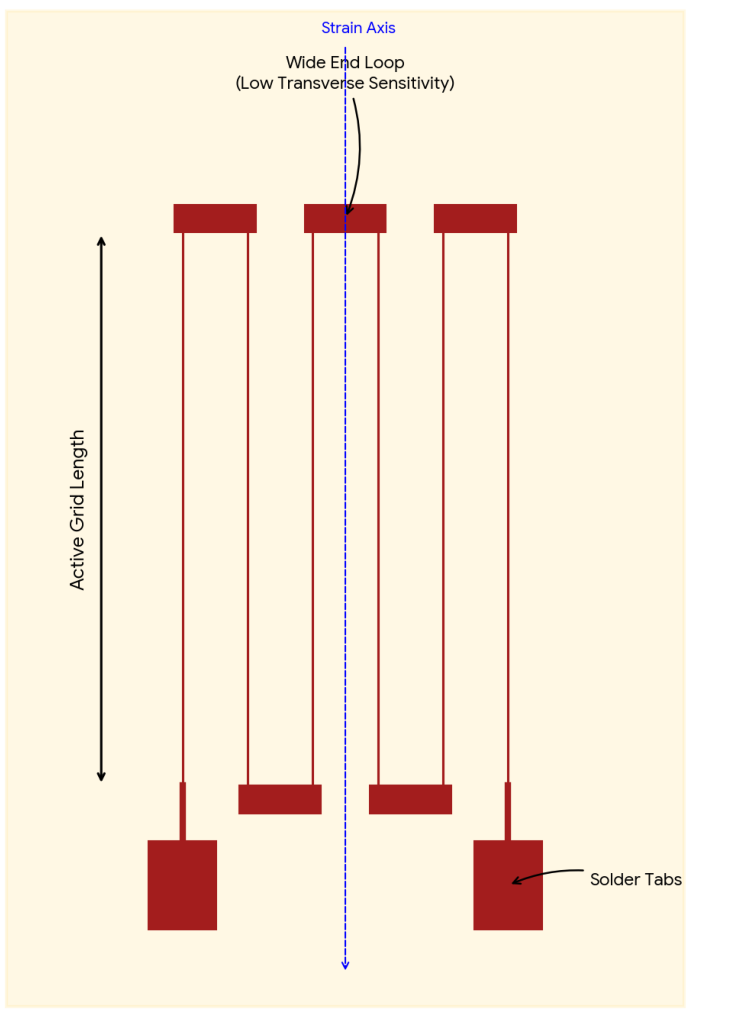
\includegraphics[height=68mm]{source_gauge_figure.png}
\captionof{figure}{Excerpt of the supplied p.~3 diagram: long axial strands, widened end loops and two solder tabs.}
\end{minipage}\hfill
\begin{minipage}[t]{0.64\linewidth}
\vspace{0pt}
The diagram depicts a continuous serpentine resistive path, not a three-dimensional inductor. Its long strands and short, wider turns contribute different fractions of the total resistance. This geometry should enter the model rather than being described only as a ``coil.''

For a uniform segment,
\[
R=\rho_e\frac{L}{A}.
\]
For homogeneous principal stretches,
\begin{equation}
\frac{R'}{R}=\frac{\rho'_e}{\rho_e}
\frac{\lambda_\parallel}{\lambda_{\perp1}\lambda_{\perp2}}.
\end{equation}
$\rho_e$ is electrical resistivity, distinct from mass density $\rho_m$ and packed log-radius $\rho$. The stretches are positive length ratios.
\end{minipage}

\subsection*{Small-strain limit and gauge factor}
Taking a first-order logarithmic differential gives
\begin{equation}
\frac{\Delta R}{R}\simeq
\frac{\Delta\rho_e}{\rho_e}+\epsilon_\parallel-\epsilon_{\perp1}-\epsilon_{\perp2}.
\end{equation}
Under isotropic uniaxial stress, $\epsilon_{\perp1}=\epsilon_{\perp2}=-\nu\epsilon_\parallel$, so
\begin{equation}
GF=\frac{\Delta R/R}{\epsilon_\parallel}
\simeq1+2\nu+\frac{\Delta\rho_e/\rho_e}{\epsilon_\parallel}.
\end{equation}
For a grid with unit strand direction $\bm a$, the directional substrate strain is $\epsilon_a=\bm a^T\bm\epsilon\bm a$. A bonded gauge also needs a strain-transfer factor or calibrated transfer model for its adhesive and backing. Metallic gauges commonly have $GF$ near two, but the actual factor is a specimen input. [R7]

\subsection*{Weighted grid and semiconductor extension}
For trace segments connected in series,
\begin{equation}
R_{\rm grid}=\sum_iR_i,\qquad
\frac{\Delta R_{\rm grid}}{R_{\rm grid}}
=\sum_i\frac{R_i}{R_{\rm grid}}\frac{\Delta R_i}{R_i}.
\end{equation}
Widened returns reduce their resistance weighting; they do not make transverse sensitivity identically zero. For crystalline gauges, add a stress-dependent resistivity model, for example $\Delta\rho_{ij}/\rho_0=\pi_{ijkl}\sigma_{kl}$ in the specified crystal frame. The coefficients $\pi_{ijkl}$, temperature and doping are calibration/material data, not consequences of the meander's appearance.

\newpart
\section{Correct Wheatstone bridge law and exact inversion}
\label{sec:bridge}
\src{[S2], p.~5: exact bridge formula and quarter-bridge approximation}

Declare two voltage dividers. $R_1$ is upper left, $R_2$ lower left, $R_3$ upper right and $R_4$ lower right. The upper nodes are at $V_{\rm ex}>0$ and lower nodes at zero. Measure $V_o=V_L-V_R$. Kirchhoff's laws give
\begin{equation}
v:=\frac{V_o}{V_{\rm ex}}
=\frac{R_2}{R_1+R_2}-\frac{R_4}{R_3+R_4}.
\label{eq:bridge}
\end{equation}
This preserves the terminal convention in the supplied equation, with $R_4=R_x$. The two-divider interpretation is also the standard bridge construction. [R7]

\begin{center}
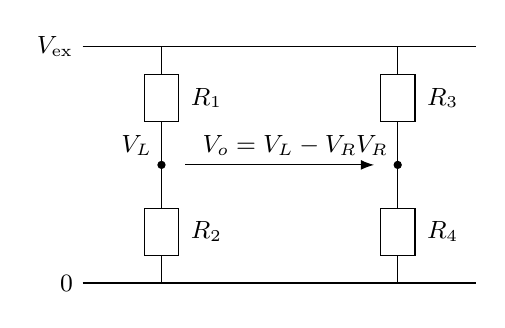
\begin{tikzpicture}[x=1cm,y=1cm,>=Latex, every node/.style={font=\small}]
\draw (0,0)--(5,0);\draw (0,3)--(5,3);
\node[left] at (0,3){$V_{\rm ex}$};\node[left] at (0,0){$0$};
\foreach \x/\top/\bot/\lab in {1/R_1/R_2/V_L,4/R_3/R_4/V_R}{
\draw (\x,3)--(\x,2.65);\draw (\x-.22,2.05) rectangle (\x+.22,2.65);
\draw (\x,2.05)--(\x,.95);\draw (\x-.22,.35) rectangle (\x+.22,.95);\draw (\x,.35)--(\x,0);
\node[right] at (\x+.25,2.35){$\top$};\node[right] at (\x+.25,.65){$\bot$};
\fill (\x,1.5) circle(1.5pt);\node[above left] at (\x,1.5){$\lab$};}
\draw[->] (1.3,1.5)--(3.7,1.5) node[midway,above]{$V_o=V_L-V_R$};
\end{tikzpicture}
\end{center}

\subsection*{Quarter bridge}
Set $R_1=R_2=R_3=R$ and $R_4=R(1+x)$, with $x>-1$. Then
\begin{equation}
\boxed{\ v=-\frac{x}{4+2x},\qquad x=-\frac{4v}{1+2v}\ },
\qquad -\tfrac12<v<\tfrac12.
\label{eq:quarter}
\end{equation}
For an isothermal, linear calibrated gauge, $x=GF\epsilon$ and
\begin{equation}
V_o\simeq-\frac{V_{\rm ex}GF\epsilon}{4}.
\end{equation}
The positive sign on [S2, p.~5] therefore requires reversing the measurement leads or changing the active arm. It does not follow from that page's stated exact formula. Retaining this polarity throughout prevents a feedback controller from responding in the wrong direction.

\subsection*{Linearization error and multiple active arms}
The signed relative error of replacing $-x/(4+2x)$ by $-x/4$, measured relative to the exact nonzero output, is $x/2$; its magnitude is $|x|/2$. A larger $GF$ can therefore make bridge nonlinearity relevant at a smaller strain. For $R_i=R(1+x_i)$,
\begin{equation}
v\simeq\frac{-x_1+x_2+x_3-x_4}{4}.
\end{equation}
This formula fixes the signs of all half- and full-bridge arrangements before any gain or thermal-cancellation claim is made.

\newpart
\section{Thermal compensation, self-heating and sensitivity}
\label{sec:bias}
\src{[S2], pp.~5--6; [S0], PDF pp.~13--17}

\subsection*{A transverse gauge is not automatically a dummy}
Under uniaxial stress in an isotropic specimen,
\begin{equation}
\epsilon_\perp=-\nu\epsilon_\parallel.
\end{equation}
With axial $R_4$ and bonded transverse $R_3$, equal factors give $x_4=GF\epsilon$ and $x_3=-GF\nu\epsilon$. Hence the declared bridge polarity gives
\begin{equation}
v\simeq-\frac{GF(1+\nu)\epsilon}{4}.
\end{equation}
The transverse gauge contributes signal. A mechanical dummy instead has negligible load strain while sharing the relevant temperature; the source's bonded-transverse description does not establish that condition. NI explicitly distinguishes these configurations. [R7]

A common multiplicative change of \emph{all} arm resistances leaves equation~\eqref{eq:bridge} unchanged exactly. More limited cancellation requires matched temperature coefficients, matched temperatures and an appropriate arm arrangement. Thermal gradients, adhesive expansion and lead resistance can remain.

\subsection*{Separate mechanical signal from temperature}
A selected calibration model for each installed gauge is
\begin{equation}
x(\epsilon,T)=GF_0\epsilon+c_T\Delta T+c_{\epsilon T}\epsilon\Delta T
+c_2\epsilon^2+c_0,\qquad \Delta T=T-T_0.
\label{eq:gaugecal}
\end{equation}
This is a fitted constitutive approximation, not a material law with universal coefficients. For a quarter bridge with the other three arms fixed at the reference resistance, obtain $x$ from the exact inverse before removing the fitted temperature and offset terms. With multiple varying arms, fit the full divider equation instead. Measure the actual excitation voltage to form the ratio $v$.

At balance, each arm dissipates
\begin{equation}
P_g=\frac{V_{\rm ex}^2}{4R},\qquad
P_{\rm bridge,total}=\frac{V_{\rm ex}^2}{R}.
\end{equation}
For $R=350\,\Omega$, one arm dissipates $0.7143$ mW at 1 V and $7.7786$ mW at 3.3 V. These are calculated values. Only the heat of arms physically coupled to the specimen enters its local thermal model. Reducing excitation lowers signal linearly but Joule heating quadratically.

\subsection*{Measurement is a physical perturbation}
For a scalar steady thermal path, $\Delta T_{\rm bias}=P_{\rm coupled}/G_{\rm th}$. This can alter the lens, the reporter and the thermochromic coating. Pulsed excitation is an option, but its duty cycle, electrical settling and thermal transient must all be included.

A semiconductor gauge with an assigned larger $GF$ does not by itself remove the need for an amplifier or temperature measurement. Compare the complete transfer function with input-referred noise, required bandwidth, drift, headroom and calibration residual. The source's foil-versus-semiconductor voltage categories are not universal.

\newpart
\section{The vertical slit as a real optical operator}
\label{sec:slit}
\src{[S1], pp.~3--4; [S0], PDF p.~12}

\subsection*{Aperture geometry}
In an aperture plane, choose orthogonal in-plane unit directions $\bm a$ across the slit and $\bm b$ along it. Let its centre be $\bm r_c$, width $w_s>0$ and height $h_s>0$. Define the binary amplitude aperture
\begin{equation}
A(\bm r)=\ind\{|\bm a\!\cdot(\bm r-\bm r_c)|\le w_s/2\}
\ind\{|\bm b\!\cdot(\bm r-\bm r_c)|\le h_s/2\}.
\end{equation}
A tilt changes the plane/frame; a shift changes $\bm r_c$. Deformation changes the edge locations according to the mechanical model. These are independent parameters, not automatic results of using an elongated pupil. Pupil-shape research supports orientation-dependent optical behavior, not equivalence between a pupil and a leaf rim. [R2]

\begin{proposition}[Slit restriction]
On a scalar field $U$, define $\mathsf P_AU=AU$. Then
\begin{equation}
\mathsf P_A^2=\mathsf P_A,\qquad
\int|\mathsf P_AU|^2\dd A\le\int|U|^2\dd A.
\end{equation}
\end{proposition}
\begin{proof}
The indicator satisfies $A^2=A$ and $0\le A\le1$ pointwise. Multiply by $U$, then integrate the squared magnitude.
\end{proof}
This is a precise mathematical role for the slit: it selects a field region without creating optical power. A real coating with complex transmission $t_\lambda$ is not generally an idempotent projection.

\subsection*{Transmission, lens phase and propagation}
A selected scalar optical model is
\begin{equation}
U_{{\rm det},\lambda}
=\mathsf H_{z,\lambda}
\big[A\,t_\lambda(T,a,\zeta)\,
\exp(i\varphi_{\rm lens,\lambda})U_{{\rm in},\lambda}\big].
\end{equation}
$\mathsf H$ is a declared diffraction propagator, or its experimentally calibrated transfer. The physical optics can be characterized offline and compiled into a lookup table. The parent kernel can still avoid ray tracing, ray marching and coordinate squaring at runtime; that instruction choice does not remove diffraction from the physical device.

For a uniformly illuminated rectangular slit in the Fraunhofer regime, with vacuum wavelength $\lambda$ and propagation-medium index $n_m$, the first-zero angles satisfy
\begin{equation}
\sin\alpha_x=\lambda/(n_mw_s),\qquad \sin\alpha_y=\lambda/(n_mh_s)
\end{equation}
when those ratios are at most one. A narrower slit increases diffraction across its narrow direction. These relations follow from the zeros of the Fourier transform of a rectangle; they are not a guarantee of sharper focus in every regime.

\newpart
\section{Liquid lensing, two bands and absorbed energy}
\label{sec:optics}
\src{[S1], p.~4, ``variable convexity'' and ``dichromatic funneling''}

\subsection*{A liquid lens needs its own constitutive model}
At a static interface, Snell's law is $n_1\sin\theta_1=n_2\sin\theta_2$. A fluid interface at mechanical equilibrium also obeys the Young--Laplace pressure jump,
\begin{equation}
\Delta p=\gamma\left(\frac1{\mathcal R_1}+\frac1{\mathcal R_2}\right).
\end{equation}
Here the signed principal radii belong to the fluid surface. In a thin, paraxial lens surrounded by the same medium on both sides,
\begin{equation}
\frac1{f_\lambda}=\left(\frac{n_\ell(\lambda)}{n_m(\lambda)}-1\right)
\left(\frac1{R_{\rm front}}-\frac1{R_{\rm back}}\right).
\end{equation}
The front/back radii use one declared optical sign convention. Contact angle, pressure or another actuator sets the shape. Electrowetting-controlled focal length has an experimental literature; its existence does not determine a focal law for the supplied geometry. [R3]

A slit aperture is not automatically a waveguide and does not force the lens edge to become more convex. Those behaviors require a specified material/interface and a solved or measured shape. A static passive lens changes propagation direction and intensity distribution, not the energy of an individual photon at fixed frequency.

\subsection*{Two spectral channels are not one binary measurement}
Let $\lambda$ denote vacuum wavelength and $P_\lambda$ incident spectral power at a declared input plane in $\mathrm{W\,m^{-1}}$ of wavelength. Let $\tau_k(\lambda)$ be the fraction delivered to channel $k$ and $\eta_k(\lambda)$ its quantum efficiency. For an exposure interval,
\begin{equation}
\mu_k=\int_{t_n}^{t_{n+1}}\int
\eta_k(\lambda)\tau_k(\lambda)P_\lambda(t)
\frac{\lambda}{hc}\dd\lambda\dd t,\qquad k=1,2.
\end{equation}
The observations include background and readout noise. The bands and response curves are calibrated inputs. For nonoverlapping branches of a passive splitter, the power fractions must share one energy budget; they are not two copies of the incident power.

Two channel counts remain two observables. A later rule produces the one-bit event. In single-photon mode, requiring a count in \emph{both} nonoverlapping spectral branches would reject an ideally routed single photon; use a declared primary score or band selection instead.

\subsection*{Absorption ledger}
For a passive incident-light interaction, at a specified wavelength and geometry,
\begin{equation}
\mathcal R_\lambda+\mathcal T_\lambda+\mathcal A_\lambda=1,
\qquad P_{\rm abs}=\int\mathcal A_\lambda P_\lambda\dd\lambda .
\end{equation}
Here reflection and transmission include their relevant outgoing directions. Stored excitation, emitted light, electrical extraction and subsequent heat must be accounted for after absorption; absorption is not necessarily instantaneous conversion of all energy into heat.

\newpart
\section{The eye-inspired material witness}
\label{sec:witness}
\src{[S1], pp.~3,5--7: cellulose/jelly, double verification and quantum sensing}

The optical analogy has two distinct realizations. Retinal phototransduction begins with a pigment's light-induced molecular change and subsequent biochemical amplification; rod responses and behavioral detection are different levels of observation. Single-photon rod responses and probabilistic human single-photon detection have been experimentally studied. Neither establishes cellulose combustion as the mechanism of an eye. [R5,R6]

The transferable proposal is instead an \textbf{engineered material-state witness}: a change of a specified absorber or reporter that accompanies an optical interaction. A cellulose-containing hydrogel may be retained as a proposed supporting matrix. Its formulation, absorber, reaction pathway, response time and regeneration mechanism are not specified by the supplied files.

\subsection*{A minimal, bounded reporter model}
Define $\zeta\in[0,1]$ as the fraction of reporter sites in the changed state. A chosen two-state kinetic model is
\begin{equation}
\dot\zeta=k_+(1-\zeta)-k_-\zeta,\qquad k_+,k_-\ge0.
\end{equation}
One candidate photoactivation rate is $k_{\rm ph}=\int Y_\lambda\sigma_\lambda\Phi_\lambda\dd\lambda$, where $\Phi_\lambda$ is photon flux per area and wavelength, $\sigma_\lambda$ an absorption cross-section, and $Y_\lambda$ the conversion yield. Other activation and recovery processes enter $k_+$ and $k_-$. Their measured values determine the model, not the word ``burn.''

For constant rates during a step, let $k=k_++k_-$. When $k>0$,
\begin{equation}
\zeta_{n+1}=\frac{k_+}{k}
+\left(\zeta_n-\frac{k_+}{k}\right)e^{-k\Delta t};
\qquad k=0:\quad\zeta_{n+1}=\zeta_n.
\label{eq:reporter}
\end{equation}
Both the equilibrium and initial state lie in $[0,1]$, and this update is their convex combination. It therefore preserves the state interval exactly. A readout $Y$ can be formed from a calibrated change in fluorescence, resistance, temperature or another specified observable; the present documents do not select one.

\subsection*{Declare what the second channel actually verifies}
\small
\begin{tabularx}{\linewidth}{@{}P{10mm}P{40mm}Y@{}}
\toprule
\textbf{Mode} & \textbf{Profile name} & \textbf{Meaning of the accepted event}\\
\midrule
0 & Geometry-qualified optical & Optical evidence while strain/aperture state is acceptable. Strain qualifies geometry; it is not a second proof of photon absorption.\\
1 & Absorber-coupled pulse & A primary optical/electrical pulse with a matching absorber-linked thermal or other physical response. The calibrated pulse-energy range is explicit.\\
2 & Material-state reporter & Primary evidence plus a changed reporter state. Recovery, accumulated dose and prior history enter the gate.\\
3 & Characterized single photon & A separately characterized single-photon instrument and its recorded auxiliary evidence. Photon-number response, dark events and timing are measured.\\
\bottomrule
\end{tabularx}
\normalsize
These are new profile definitions, not measured performance levels. Recovery or replacement of the material consumes time and may consume supplied energy. A downstream reporter cannot absorb the entire same photon after that photon was already destroyed in a separate primary absorber.

\newpart
\section{Double verification as a statistical operator}
\label{sec:gate}
\src{[S1], pp.~5--7; the definitions and probability derivations below are new}

Let $H_0$ mean no event of the selected profile and $H_1$ mean its declared event. Let $X,Y$ be thresholded primary and secondary evidence; $C_t$ a timing-match bit; $V$ record validity; $S$ saturation; and $F$ a fault bit. Each is in $\bb$. Define
\begin{equation}
\boxed{\ e=X\land Y\land C_t\land V\land\neg S\land\neg F\ }.
\label{eq:gate}
\end{equation}
A lag-corrected timing gate is
\begin{equation}
C_t=\ind\{|(t_Y-t_X)-\tau_{\rm lag}|\le\Delta_c/2\}.
\end{equation}
The delay and window are calibrated for the chosen material and readout. A slow thermal response can verify an integrated pulse; it does not automatically identify one photon among many arrivals during its integration time.

\subsection*{What two observations can and cannot guarantee}
With all quality and timing conditions satisfied, the false-acceptance probability obeys
\begin{align}
p_{\rm FA}&=P(X=1,Y=1\mid H_0)\\
&=\alpha_X\alpha_Y+\operatorname{Cov}(X,Y\mid H_0),
\quad \alpha_X=P(X=1\mid H_0),\quad\alpha_Y=P(Y=1\mid H_0),\\
0&\le p_{\rm FA}\le\min(\alpha_X,\alpha_Y).
\end{align}
Only conditional independence removes the covariance term. Shared temperature drift, supply interference, scattered light or copied software flags can create common-mode errors. If $Y$ is a deterministic function of $X$, it adds no conditional information about the event: $I(H;Y\mid X)=0$.

The same intersection also reduces detection probability. Under conditional independence, $p_D=p_{D,X}p_{D,Y}$; values $0.95$ and $0.90$ give $0.855$, not perfect detection. The full gate is calibrated jointly, including quality conditions; conditional channel rates must not be mixed with unconditional system rates.

For independent stationary Poisson background streams with rates $r_X,r_Y$, counting every pair whose separation lies in a window of total width $\Delta_c$ gives
\begin{equation}
r_{\rm pair}=r_Xr_Y\Delta_c.
\end{equation}
If each $X$ trigger is counted only once when at least one $Y$ lies in its window, the expected trigger rate is instead $r_X(1-e^{-r_Y\Delta_c})$. Dead time and non-Poisson correlations require a different model.

\subsection*{Evidence for a small false-acceptance rate}
For $N$ independent, identically distributed null trials with zero accepted events, the one-sided confidence-$1-\alpha$ upper bound is
\begin{equation}
p_{\rm FA,upper}=1-\alpha^{1/N}.
\label{eq:zerofail}
\end{equation}
This follows by solving $(1-p)^N=\alpha$. Zero events in $10{,}000$ trials give a 95\% upper bound of about $2.9953\times10^{-4}$ per trial. A finite no-failure test therefore establishes a bound, not absolute zero false positives.

\newpart
\section{A quantum-instrument extension of Operator I}
\label{sec:quantum}
\src{[S1], pp.~6--7, the request to extend the idea to quantum sensing}

For a photon-resolved profile, the physical measurement can be specified as a quantum instrument rather than inferred from the binary output. The mathematical instrument framework describes outcome probabilities and the associated state changes. [R13]

Let $\varrho_Q\succeq0$, $\tr\varrho_Q=1$ be the optical input density operator, including any explicitly modeled auxiliary system. It is distinct from the packed log-radius $\rho$. Choose outcome operators $K_{j\ell}$ satisfying
\begin{equation}
\sum_{j,\ell}K_{j\ell}^{\dagger}K_{j\ell}=\bm1.
\end{equation}
Define the outcome map, probability and conditional state by
\begin{equation}
\mathcal J_j(\varrho_Q)=\sum_\ell K_{j\ell}\varrho_QK_{j\ell}^{\dagger},
\quad p_j=\tr\mathcal J_j(\varrho_Q),
\quad\varrho_{Q|j}=\mathcal J_j(\varrho_Q)/p_j
\end{equation}
for $p_j>0$. The outcome record $j$ may include both sensors, a timing bin and quality flags. Operator I applies the classical gate $g(j)$ from equation~\eqref{eq:gate}:
\begin{equation}
\mathcal J_{e}(\varrho_Q)=\sum_{j:g(j)=e}\mathcal J_j(\varrho_Q),
\qquad P(e)=\tr\mathcal J_e(\varrho_Q).
\end{equation}

\begin{proposition}[Normalized event instrument]
The coarse-grained event maps are completely positive and trace non-increasing, and $P(e=0)+P(e=1)=1$.
\end{proposition}
\begin{proof}
Each map is a sum of operator-sandwich terms and therefore completely positive. The completeness relation gives $\sum_j\tr\mathcal J_j(\varrho_Q)=\tr\varrho_Q=1$. Partitioning the outcomes into $g(j)=0$ and $g(j)=1$ preserves this sum, and each nonnegative part is at most one.
\end{proof}

\subsection*{One absorption, potentially several readouts}
Several macroscopic signals may originate in one absorbed-energy event. Their correlations and supplied amplification energy belong in the instrument and energy model. They are not multiple independent copies of the full incident photon energy. A destructive absorption also changes the optical state, so repeatability must be defined for the detector record rather than assumed for the original photon.

NIST describes superconducting transition-edge sensors that resolve the temperature change associated with photon absorption under specialized cryogenic operating conditions. That is a physically established route to a thermal photon witness, separate from an unspecified ambient cellulose matrix. [R9]

The operators $K_{j\ell}$ are model inputs to be characterized; they have not been measured for this proposed device. A claim of quantum advantage would additionally require a stated estimation task, resources and comparison baseline. The present extension supplies an instrument specification into which such evidence can be placed.

\newpart
\section{Energy closure and thermochromic feedback}
\label{sec:thermal}
\src{[S0], PDF pp.~13--17; [S1], pp.~5--7; [S2], p.~6}

\subsection*{One energy ledger for every coupled mechanism}
For a fixed material system with its energy stores explicitly partitioned, write the first law over an interval as
\begin{equation}
\Delta(U_{\rm th}+E_{\rm elastic}+K_{\rm mech}+E_{\rm chem})
=E_{\rm abs}+E_{\rm electrical}+W_{\rm ext}-Q_{\rm bath}-E_{\rm other,out}.
\end{equation}
Unabsorbed reflected/transmitted light is already excluded from $E_{\rm abs}$. $E_{\rm other,out}$ contains any energy subsequently exported as luminescence, electricity or another separately specified channel. A consistent thermoelastic free-energy model must avoid counting coupled thermal/elastic storage twice.

A selected reduced thermal node model is
\begin{align}
C_i\dot T_i={}&P_{{\rm heater},i}+P_{{\rm bridge},i}+P_{{\rm abs\to heat},i}
+P_{{\rm chem\to heat},i}+P_{{\rm mech\to heat},i}\notag\\
&-G_{i0}(T_i-T_a)-\sum_jG_{ij}(T_i-T_j),
\label{eq:thermal}
\end{align}
where $C_i>0$, $G_{ij}=G_{ji}\ge0$, and $G_{i0}\ge0$. The chemical and mechanical heat terms are internal transfers from explicitly tracked stores or dissipation of supplied work. They are not independent new energy sources. A model using all absorbed power as immediate heat must not add the same delayed relaxation heat a second time.

For one node with constant net applied heat $P$, $C$ and $G>0$,
\begin{equation}
T_{n+1}=T_a+P/G+(T_n-T_a-P/G)e^{-G\Delta t/C}.
\label{eq:thermalstep}
\end{equation}
This exact step is useful for pulse-response calibration and avoids the step-size instability of a careless explicit Euler update. The spatial parent model remains available when one thermal node is insufficient.

\subsection*{Hysteresis is material memory, not a word inversion}
Retain the parent's calibrated two-threshold darkness model. For $T_{\rm low}<T_{\rm high}$, a selected idealized state $a$ follows
\begin{equation}
a_{n+1}=\begin{cases}
1,&T_{n+1}\le T_{\rm low},\\
0,&T_{n+1}\ge T_{\rm high},\\
a_n,&T_{\rm low}<T_{n+1}<T_{\rm high}.
\end{cases}
\end{equation}
A measured darkness bit $D$ is obtained from optical reflectance/transmittance and its threshold; it need not equal this ideal state on every noisy observation. Thermochromic color and phase behavior depend on the actual composite. [R14; S0, PDF p.~15.]

The Klein bit changes a logical mapping; it does not reverse a passive thermal conductance or supply heat-pump work. Likewise, the Landauer lower bound $k_BT\ln2$ concerns erasure of an unknown, unbiased bit in its standard isothermal setting, not a fixed heat payment for every XOR, shift or bit flip. The corrected parent energy-accounting distinction is retained. [S0, PDF p.~14; R15]

\newpart
\section{Deformation-aware PSI pruning}
\label{sec:psi}
\src{[S0], PDF p.~12, descendant-enclosure condition; [S1], rim geometry; [S2], strain}

The physical rim and aperture can move. A PSI bound must consequently enclose deformed descendants, not only their undeformed centers. Let a slit be the slab
\begin{equation}
\mathcal A_s=\{\bm x:|\bm n\cdot\bm x-c|\le w_s/2\},\qquad\|\bm n\|=1.
\end{equation}
Suppose the entire relevant undeformed descendant set obeys
$|\bm n\cdot(\bm X-\bm P)|\le R_N$. Also suppose projected deformation is bounded by $d_N$ and all remaining projected encoding/alignment uncertainty by $\delta_N$.

\begin{proposition}[Conservative deformed-slit exclusion]
If
\begin{equation}
\boxed{\ |\bm n\cdot\bm P-c|>w_s/2+R_N+d_N+\delta_N\ },
\label{eq:psi}
\end{equation}
no enclosed physical descendant intersects the slit slab during the certified interval.
\end{proposition}
\begin{proof}
For a represented point $\bm x=\bm P+(\bm X-\bm P)+\bm u+\bm e$, the reverse triangle inequality gives
\[
|\bm n\cdot\bm x-c|\ge|\bm n\cdot\bm P-c|-R_N-d_N-\delta_N>w_s/2.
\]
The assumptions apply to every descendant and every time in the interval, so the exclusion applies to the entire certified set.
\end{proof}

Equality is not excluded. The radius $R_N$ must bound all descendants to be removed, including transformed children; a depth counter by itself is not such a bound. Deformation estimates require an uncertainty margin. A later Klein return to a new root is a new evaluation epoch, not an excuse to discard future state updates forever.

For rounded log-radius spacing $\Delta\rho$, a useful upper relative radial encoding error is $2^{\Delta\rho/2}-1$. Rounded 2048-bin phase has maximum angular error $\pi/2048$. Convert these and mounting uncertainties into a length bound for the relevant physical scale before adding them in equation~\eqref{eq:psi}.

\subsection*{Geometric exclusion is not thermal or optical silence}
Diffraction and scattering can couple fields across a geometrical boundary. Heat can cross it through the connected substrate. Therefore an occupancy-pruned node is not automatically removed from the physical forward model. Bound its omitted optical contribution by a declared optical-error budget and its omitted heating by a separate thermal budget.

For a constant-capacitance passive linear thermal network, an additional nonnegative omitted heat input of cumulative energy $E_{\rm omit}$, starting from zero temperature difference between two runs with all other inputs equal, satisfies
\begin{equation}
0\le\Delta T_i\le E_{\rm omit}/C_i.
\end{equation}
The network preserves nonnegative temperature increments; summing its incremental energy balances cancels internal conductances and leaves only nonnegative bath losses. Thus $C_i\Delta T_i\le\sum_j C_j\Delta T_j\le E_{\rm omit}$. Nonlinear feedback changes require a new bound.

\newpart
\section{Unchanged W64 core and explicit version semantics}
\label{sec:word}
\src{[S0], PDF pp.~6--12 and embedded reference implementation}

The parent word uses every bit. Sensor temperature, strain, photon-channel evidence and validity metadata remain outside it. One bit is the event output, not a claim that every physical degree of freedom is stored in one bit.

\small
\begin{tabularx}{\linewidth}{@{}P{22mm}P{18mm}P{15mm}Y@{}}
\toprule
\textbf{Bit range} & \textbf{Field} & \textbf{Width} & \textbf{Preserved interpretation}\\
\midrule
63 & $\chi$ & 1 & Symbolic channel/control label\\
62:52 & $\rho$ & 11 & Signed packed log-radius code\\
51:41 & $\theta$ & 11 & Unsigned phase modulo 2048\\
40:30 & $z$ & 11 & Signed axial code\\
29:20 & $\Phi$ & 10 & Unsigned pinion/phyllotaxis register\\
19:15 & depth & 5 & Tree depth 0--31\\
14:10 & phase & 5 & Discrete cycle phase, parent FT label\\
9:3 & LUT & 7 & Polar lookup index\\
2 & $\kappa$ & 1 & Seam parity bit\\
1:0 & cycle & 2 & Symbolic cycle selector\\
\bottomrule
\end{tabularx}
\normalsize

\subsection*{Operator profiles stay distinguishable}
The grouped parent phase generator remains
\begin{equation}
\operatorname{OTAN2}_{G0}(r,O)=\big[(r\mathbin{\&}2047)\oplus(O\ll10)\big]\mathbin{\&}2047.
\end{equation}
It is a defined integer phase map, not an inverse Cartesian angle function. The literal ungrouped left-fold profile has different semantics and only two possible outputs; it is not silently substituted. The low-three-bit parity reads cycle and seam metadata, not the coordinate sign bits.

The real-valued reference Pinion Double Hadamard map remains
\begin{equation}
A_\phi=\diag(\phi,\phi^{-1},1,-1)H_4,\qquad
H_4=\frac12
\begin{pmatrix}1&1&1&1\\1&-1&1&-1\\1&1&-1&-1\\1&-1&-1&1\end{pmatrix}.
\end{equation}
$H_4$ is orthogonal; $A_\phi$ has determinant $-1$ and preserves four-dimensional volume, not all lengths or physical energy. The parent's rational integer coefficients, rounding, clipping and modular phase rules remain authoritative for executable results.

The seam reflection uses $\theta\mapsto(1024-\theta)\bmod2048$ and $\kappa\mapsto\kappa\oplus1$. Its additional log-radius inversion is applied on the parent's symmetric code range. A double seam crossing is a logical involution; two dissipative physical cycles need not restore temperature or reporter state. Setting $\beta=0$ in section~\ref{sec:operator} retains the parent kernel exactly.

\newpart
\section{A 64-byte measurement record, separate from W64}
\label{sec:packet}
\textbf{New transport definition.} All multi-byte values are little-endian. The 64-byte record is 512 bits, including one unchanged 64-bit node word. It is not a repacking of the parent's occupied bits.

\small
\begin{tabularx}{\linewidth}{@{}P{17mm}P{32mm}P{20mm}Y@{}}
\toprule
\textbf{Bytes} & \textbf{Field} & \textbf{Type} & \textbf{Meaning / constraint}\\
\midrule
0--1 & magic & 2 bytes & ASCII \texttt{WI}\\
2, 3 & version & 2 uint8 & Major 1; minor 1\\
4--7 & sequence & uint32 & Session record number, modulo $2^{32}$\\
8--15 & tick\_ns & uint64 & Monotonic acquisition timestamp in ns\\
16--23 & word & uint64 & Parent W64 state associated with record\\
24--27 & temperature\_mK & int32 & Nonnegative absolute temperature in mK; zero invalid\\
28--31 & strain\_nano & int32 & Dimensionless strain multiplied by $10^9$\\
32--35 & band1\_counts & uint32 & Calibrated primary-band acquisition code\\
36--39 & band2\_counts & uint32 & Calibrated second-band acquisition code\\
40--43 & secondary\_counts & int32 & Secondary physical-witness summary\\
44--45 & flags & uint16 & Bit meanings below\\
46 & mode & uint8 & Profile 0--3 from section~\ref{sec:witness}\\
47 & reserved & uint8 & Must be zero\\
48--51 & calibration\_id & uint32 & Registry key; nonzero for a valid record\\
52--55 & window\_ns & uint32 & Integration duration, 1 to $2^{32}-1$ ns\\
56--59 & site\_id & uint32 & Physical pinion/sensor site identifier\\
60--63 & checksum & uint32 & CRC-32 over bytes 0--59\\
\bottomrule
\end{tabularx}
\normalsize

The timestamp identifies the end of the acquisition interval on the declared session clock. Store clock epoch, synchronization uncertainty, gains, band response curves, secondary-channel units, event lag and window, reporter history policy, and physical limits in the calibration registry. The maximum represented integration duration is about 4.295 s; longer integrations need another declared profile or multiple records, not integer wraparound.

\subsection*{Flags and receiver contract}
Bits 0--3 are $X,Y,C_t,V$. Bit 4 is accepted event $e$. Bits 5--6 are saturation and fault. Bit 7 is measured optical darkness $D$. Bits 8--10 mark temperature, strain and the paired band acquisition valid. Bits 11--15 are zero. The receiver checks that bit 4 agrees exactly with equation~\eqref{eq:gate}.

A valid flag is an acquisition assertion, not something a checksum can independently prove. The controller additionally checks calibration availability, session, freshness and required channel validity. A calibration profile may use one band as the primary score; paired acquisition does not require both bands to contain photons.

The encoder uses Python's \texttt{zlib.crc32}; its check value for \texttt{123456789} is \texttt{CBF43926}. This detects transmission errors, not malicious tampering. [R12] Out-of-range encodings are rejected. Saturated hardware measurements retain the saturation flag; they are not accepted as verified events. Acquisition ``counts'' are not photon numbers unless the instrument's calibration establishes that interpretation.

\newpart
\section{Calibration, identifiability and decisive tests}
\label{sec:calibration}

The files supply concepts, equations and software architecture, but no specimen-specific measurement series. The next physical improvement is a calibration design that separates the mechanisms rather than fitting every change to ``light.''

\small
\begin{tabularx}{\linewidth}{@{}P{34mm}Y@{}}
\toprule
\textbf{Controlled experiment} & \textbf{Quantity or distinction established}\\
\midrule
Known loads at controlled temperature & Elastic response, gauge strain transfer, bridge polarity, stiffness and load-to-voltage sensitivity.\\
Temperature sweep at specified fixed load & Gauge drift, thermal expansion, thermochromic hysteresis and temperature-dependent optical response.\\
Optical pulses at fixed geometry, heater command off & Band response, detection efficiency at a declared plane, pulse lag, reporter/thermal response and optical background.\\
Heater-only and mechanical-only trials in controlled darkness & Non-optical triggers that might imitate the secondary witness; coupling from bridge self-heating.\\
Combined inputs with randomized, held-out trials & Joint detection/false-acceptance rates, timing gate, saturation behavior and feedback stability under defined operating conditions.\\
\bottomrule
\end{tabularx}
\normalsize

\subsection*{Why independent parameter variation matters}
For equation~\eqref{eq:gaugecal}, a fitted design matrix with rows
\begin{equation}
[\,1,\ \epsilon,\ \Delta T,\ \epsilon\Delta T,\ \epsilon^2\,]
\end{equation}
must have column rank five to identify five coefficients in a noise-free linear parameter fit. Good conditioning is also needed with noise. If every illumination change causes the same linked temperature and strain changes, the observations may not separate their coefficients. A large number of repetitions at one condition does not repair that identifiability problem.

\subsection*{Uncertainty attached to an inferred strain}
For an isothermal quarter bridge, the exact estimate is
\begin{equation}
\widehat\epsilon=-\frac{4v}{GF(1+2v)},\quad
\frac{\partial\widehat\epsilon}{\partial v}=-\frac4{GF(1+2v)^2},\quad
\frac{\partial\widehat\epsilon}{\partial GF}=-\frac{\widehat\epsilon}{GF}.
\end{equation}
For input vector $\bm z$ containing $v,GF$ and the relevant thermal/calibration quantities, first-order propagation is
\begin{equation}
u_\epsilon^2\simeq J\Sigma_zJ^T,\qquad J=\partial\widehat\epsilon/\partial\bm z.
\end{equation}
Covariance terms are retained. The uncertainty budget records voltage-reference noise, offsets, drift, calibration residuals and strain transfer rather than presenting an ADC code as exact strain. This follows the measurement-uncertainty approach documented in NIST TN~1297. [R11]

\subsection*{Minimum profile information}
A testable release needs geometry and supports; material/adhesive data; calibrated gauge and bridge parameters; spectral transfer and lens-actuation response; thermal capacities and conductances; reporter kinetics where used; channel noise and timing; and explicit acceptance limits. Analog evidence should be retained beside the one-bit decision so a rejected or missing measurement remains distinguishable from a valid negative result.

\newpart
\section{Worked calculation: geometry and electrical readout}
\label{sec:numbers1}
All numerical values in sections~\ref{sec:numbers1}--\ref{sec:numbers2} are \textbf{assigned calculation inputs}, not measurements of your proposed device. The embedded reference script reproduces the numbers.

\subsection*{A section-height example}
For $h_r/t_r=10$, the upright-to-flat second-moment ratio is 100. This is the local section result from section~\ref{sec:rimproof}; support geometry, ring deformation and rib joints still determine the complete assembly's compliance.

\subsection*{Same strain, same excitation, different assigned gauge factors}
Take $\epsilon=100\,\mu\epsilon=10^{-4}$ and $V_{\rm ex}=1$ V. Assign $GF=2$ to one gauge and $GF=100$ to another, with identical ideal quarter-bridge topology. Equation~\eqref{eq:quarter} gives
\begin{align}
GF=2:\quad x&=0.0002,&V_o&=-49.9950\ \mu\mathrm V,\\
GF=100:\quad x&=0.0100,&V_o&=-2.48756\ \mathrm{mV}.
\end{align}
The magnitude ratio is about 49.756, not a universal 100. The linearization's relative error is 0.01\% in the first case and 0.5\% in the second. Whether either signal can be read without further gain depends on the chosen converter, noise, bandwidth and required uncertainty.

At $R=350\,\Omega$ and 1 V excitation, the active arm's balance dissipation is $0.7143$ mW. At 3.3 V, it is $7.7786$ mW. This is a particularly important control input when the same structure is intended to report absorbed optical heat.

\subsection*{A slit example}
Assign vacuum wavelength $\lambda=550$ nm, slit width $w_s=100\,\mu$m and height $h_s=2$ mm, with propagation index approximated by $n_m=1$. The small-angle first-zero approximations are
\begin{equation}
\alpha_x\simeq0.0055\ \mathrm{rad},\qquad
\alpha_y\simeq0.000275\ \mathrm{rad}.
\end{equation}
The narrower dimension produces the wider diffraction spread. The exact first-zero angles are the arcsines of these ratios. These are aperture diffraction estimates, not a model of a panda's full eye or a demonstrated lens assembly.

\subsection*{The photon-energy scale}
Using the SI constants $h=6.62607015\times10^{-34}$ J s and $c=299792458$ m/s, a 550 nm photon has [R10]
\begin{equation}
E_\gamma=\frac{hc}{\lambda}=3.61172\times10^{-19}\ \mathrm J
=2.25426\ \mathrm{eV}.
\end{equation}
If fully thermalized in an assigned lumped heat capacity $C=10^{-6}$ J/K, its ideal immediate temperature rise is $3.61172\times10^{-13}$ K. With the parent's illustrative $C=0.02$ J/K, the rise is $1.80586\times10^{-17}$ K. A passive focusing change does not multiply these energies. The size and noise of the actual absorbing system determine whether a thermal signature can be resolved.

\newpart
\section{Worked calculation: a pulse and its verification}
\label{sec:numbers2}

\subsection*{An absorber-coupled pulse, not a one-photon claim}
Assign an incident optical pulse of 1 mW for 5 ms, absorption fraction 0.8, thermal capacitance $C=10^{-6}$ J/K, conductance $G=10^{-4}$ W/K, and initial equilibrium at $T_a$. Assume all absorbed pulse energy thermalizes in that node and ignore other changing heat inputs. Then
\begin{align}
P_{\rm abs}&=0.8\ \mathrm{mW},& E_{\rm abs}&=4.00000\ \mu\mathrm J,\\
\tau&=C/G=10\ \mathrm{ms},&
\Delta T_{\rm peak}&=\frac{P_{\rm abs}}G\left(1-e^{-5\,\mathrm{ms}/\tau}\right)
=3.14775\ \mathrm K.
\end{align}
The heat stored at pulse end is $3.14775\,\mu$J, and heat lost to the bath during the pulse is $0.852245\,\mu$J. Their sum is the absorbed energy. At 550 nm the absorbed-energy equivalent is approximately $1.10751\times10^{13}$ photons.

This calculation supplies a pulse-scale test regime for a physical witness. It does not assign these thermal parameters to cellulose or certify the response of an unbuilt specimen. The 1 V bridge-arm heat from the preceding page is comparable to the assigned absorbed power; its stable bias must be included or its transient separately measured. Otherwise electrical self-heating could imitate the very witness intended to verify optical absorption.

\subsection*{Independence must be demonstrated, not named}
Assign independent conditional false-trigger probabilities $\alpha_X=\alpha_Y=10^{-3}$ with timing and quality conditions satisfied. Their joint false acceptance is $10^{-6}$ per trial. With independent conditional detections 0.95 and 0.90, joint detection is 0.855. Shared disturbances invalidate the multiplication assumption.

For background rates $r_X=10$ per second, $r_Y=20$ per second and a coincidence window of total width 5 ms, the expected accidental pair rate is
\begin{equation}
r_{\rm pair}=10\times20\times0.005=1\ \mathrm{s}^{-1}.
\end{equation}
This demonstrates why merely adding a second slow sensor can leave substantial false coincidence. The unique-$X$ trigger rate is instead $10(1-e^{-0.1})\simeq0.9516$ per second under the same Poisson assumptions.

\subsection*{A quantitative acceptance target}
At 95\% confidence, zero failures in $10{,}000$ independent null trials bound the per-trial false-acceptance probability by $0.000299528$. To put that zero-failure bound below $10^{-6}$ requires at least $2{,}995{,}731$ such trials. Changes of temperature, light spectrum, timing window or mechanical setup define new conditions to which this evidence may not automatically transfer.

\begin{keybox}[MEASURABLE REPLACEMENT FOR ``DOUBLE VERIFICATION'']
Report the event profile, input plane, pulse range, two physical observables, lag/window, joint false-acceptance and detection rates, saturation exclusions, uncertainty and test conditions. This makes the source's verification idea an auditable sensing specification.
\end{keybox}

\newpart
\section{Reference implementation and conformance results}
\label{sec:software}
The embedded \texttt{operator\_i\_reference.py} implements the exact bridge transfer/inverse, event truth table, measurement encoding/decoding, bounded reporter update, projected deformation test and optional event-to-branch policy. It imports the parent's embedded kernel unchanged as \texttt{wantwomban\_reference.py}.

These checks were executed during preparation of this edition. The attached JSON contains the actual results, including the calculated examples.

\small
\begin{tabularx}{\linewidth}{@{}Y P{31mm}P{35mm}@{}}
\toprule
\textbf{Executed check} & \textbf{Count / result} & \textbf{Interpretation}\\
\midrule
Parent word round-trips / field isolation & 10,000 / 10,000 & Existing field semantics preserved\\
Parent seam involutions & 2,048 & Parent seam tests pass\\
Parent transitions / OTAN2 inputs per profile & 2,000 / 4,096 & Existing kernel tests pass\\
Bridge inverse over $-0.5\le x\le0.5$ & 10,001 cases & Max error $1.12\times10^{-16}$ or less\\
Event truth table & All 64 inputs & Exactly one accepting combination\\
Record encode/decode round-trips & 1,000 records & Exact 64-byte recovery\\
Single-bit corruption of one record & All 512 bits & Every corruption rejected\\
Bounded constant-rate reporter updates & 1,000 cases & All remain in $[0,1]$\\
Random projected descendant envelopes & 2,000 cases & 1,618 pruned enclosures\\
Points sampled within pruned enclosures & 40,450 & No sampled slit intersection\\
Parent compatibility / event-branch policy & 1,000 / 1,000 & Exact equality with specified parent calls\\
CRC check vector & CBF43926 & Matches reference function\\
\bottomrule
\end{tabularx}
\normalsize

The enclosure samples test implementation consistency; the all-points justification is the proof in section~\ref{sec:psi}, not the finite sample. The CRC test concerns single-bit corruption of one packet, not every possible multi-bit error or deliberate forgery. Software conformance is not an experiment demonstrating optical, chemical or single-photon performance.

\subsection*{Reproduction}
Extract the two Python files to one directory and run:
\begin{lstlisting}
python operator_i_reference.py
\end{lstlisting}
The script uses the Python standard library and writes \texttt{operator\_i\_results.json} beside itself. It validates ranges instead of silently inserting invalid values into neighboring bit fields. The full material, mechanical and optical equations in this document remain parameterized physical models; a finite-element solver, instrument driver and fitted quantum-instrument model are not claimed as part of this reference script.

\subsection*{Result of this sub-version}
Operator I now has typed inputs, a causal update order, measurable outputs, a preserved core, a transport contract and testable criteria. The rim, slit and gauge are connected through deformation and energy rather than through a shared visual analogy alone. The main new formal objects are the interaction operator, the material/event profiles, the deformed PSI bound and the auditable joint-event gate.

\newpart
\appendix
\section{Source provenance and embedded materials}
\label{sec:provenance}
The framework attribution is preserved as supplied: \textbf{Tom Klootwijk, NL200678942, 10-07-1990}. The parent version is 1.0; this development edition is 1.1, \textbf{WANTWOMBAN | Operator I}. The attribution and date are preserved as project metadata supplied by the author.

\small
\begin{tabularx}{\linewidth}{@{}P{12mm}Y P{22mm}@{}}
\toprule
\textbf{Key} & \textbf{Embedded source file} & \textbf{Extent}\\
\midrule
S0 & \texttt{WANTWOMBAN.pdf} & 25 pages\\
S1 & \texttt{lily pad upwards rims.pdf} & 7 pages\\
S2 & \texttt{strain gauge coil mechanism geometrically.pdf} & 6 pages\\
S3 & \texttt{Pasted markdown.md} & Original text\\
\bottomrule
\end{tabularx}
\normalsize

Page citations use physical PDF page order, counting each cover as page 1. The p.~3 foil-grid figure from S2 is reproduced as an attributed excerpt; it is not presented as a newly designed prototype. Original source files are attached byte-for-byte, including statements revised in the change register.

\subsection*{Source SHA-256 fingerprints}
\small
\textbf{S0}\par\texttt{cc0d81471fe33497873faa6339aa487532c8861902761994d3c88b16c17ea662}

\textbf{S1}\par\texttt{8041a9018ac3eafc0e3867a3de80bbb3aad0f642f0125341b641608881e6d673}

\textbf{S2}\par\texttt{1ea40e5a40660f51b9d40a86c2c07007b02c5a5b5cdbd7e72627b4702af618a3}

\textbf{S3}\par\texttt{1869efeab782774dd7af09cc2ca9e4dfd7f0317acf1549a375bbb4f8cb53d136}
\normalsize

\subsection*{Reproducible supporting files}
\texttt{wantwomban\_reference.py} is the unchanged kernel extracted from S0. \texttt{operator\_i\_reference.py} is the new extension. \texttt{operator\_i\_results.json} records the executed checks and numerical calculations. \texttt{operator\_i\_manifest.json} records source and software byte counts and SHA-256 fingerprints. The editable LaTeX source and the source-figure excerpt are also embedded.

The physical source files do not provide an assembled device, material recipe, raw calibration series or detector response measurements. Assigned examples are labeled calculations; proposed constitutive laws are labeled models; corrected source claims are recorded explicitly rather than changed inside the original attachments.

\newpart
\section{References and external grounding}
\label{sec:refs}
The source keys S0--S3 refer to the embedded documents described in Appendix~\ref{sec:provenance}. The references below supply physical and measurement context. Equations labeled as new definitions or propositions are developed in this edition; citing a physical precedent does not assert that it validates the whole proposed assembly. Online records were checked during preparation on 15 September 2026; publisher abstracts/records are used where full text was not available.

\small
\begin{description}[leftmargin=12mm,labelwidth=10mm,labelsep=2mm,itemsep=8pt]
\item[{[R1]}] Box, F., Erlich, A., Guan, J. H., and Thorogood, C. (2022). ``Gigantic floating leaves occupy a large surface area at an economical material cost.'' \emph{Science Advances} 8, eabg3790. \href{https://doi.org/10.1126/sciadv.abg3790}{doi:10.1126/sciadv.abg3790}. Primary study of giant-leaf structural economy.
\item[{[R2]}] Banks, M. S., Sprague, W. W., Schmoll, J., Parnell, J. A. Q., and Love, G. D. (2015). ``Why do animal eyes have pupils of different shapes?'' \emph{Science Advances} 1, e1500391. \href{https://doi.org/10.1126/sciadv.1500391}{doi:10.1126/sciadv.1500391}. Pupil shape, orientation and visual-function analysis; not a specification of the proposed device.
\item[{[R3]}] Berge, B., and Peseux, J. (2000). ``Variable focal lens controlled by an external voltage: An application of electrowetting.'' \emph{European Physical Journal E} 3, 159--163. \href{https://doi.org/10.1007/s101890070029}{doi:10.1007/s101890070029}. Publisher abstract/record; electrically controlled liquid-lens precedent.
\item[{[R4]}] Kelling, A. S., Snyder, R. J., Marr, M. J., Bloomsmith, M. A., Gardner, W., and Maple, T. L. (2006). ``Color vision in the giant panda (\emph{Ailuropoda melanoleuca}).'' \emph{Learning \& Behavior} 34, 154--161. \href{https://doi.org/10.3758/BF03193191}{doi:10.3758/BF03193191}. Behavioral color discrimination; not measured cone spectral curves.
\item[{[R5]}] Baylor, D. A., Lamb, T. D., and Yau, K. W. (1979). ``Responses of retinal rods to single photons.'' \emph{Journal of Physiology} 288, 613--634. \href{https://doi.org/10.1113/jphysiol.1979.sp012716}{doi:10.1113/jphysiol.1979.sp012716}. Primary electrophysiological study.
\item[{[R6]}] Tinsley, J. N., et al. (2016). ``Direct detection of a single photon by humans.'' \emph{Nature Communications} 7, 12172. \href{https://doi.org/10.1038/ncomms12172}{doi:10.1038/ncomms12172}. Probabilistic behavioral single-photon experiment.
\item[{[R7]}] NI. ``Measuring Strain with Strain Gages.'' Official measurement documentation, \href{https://www.ni.com/en/shop/data-acquisition/sensor-fundamentals/measuring-strain-with-strain-gages.html}{NI source page}. Gauge factors, bridge configurations and the distinction between a thermal dummy and a bonded transverse gauge. Exact sign and inverse calculations in this edition follow the explicitly declared divider convention.
\item[{[R8]}] S\"onnerlind, H. (2015). ``Modeling Linear Elastic Materials -- How Difficult Can It Be?'' COMSOL, 29 June 2015. \href{https://www.comsol.com/blogs/modeling-linear-elastic-materials-how-difficult-can-it-be}{Official technical article}. Linear elastic constitutive tensors and material symmetry.
\end{description}

\newpart
\section*{References / continued}
\begin{description}[leftmargin=12mm,labelwidth=10mm,labelsep=2mm,itemsep=9pt]
\item[{[R9]}] NIST, Physical Measurement Laboratory. ``Single-Photon Detectors.'' \href{https://www.nist.gov/pml/productsservices/quantum-networks-nist/technologies-quantum-networks/single-photon-detectors}{Official laboratory technology description}. Transition-edge and other detectors; thermal single-photon readout requires a specified detector and operating regime.
\item[{[R10]}] BIPM. ``SI defining constants.'' \href{https://www.bipm.org/en/measurement-units/si-defining-constants}{Official SI reference}. Exact defining values of the Planck constant, speed of light, elementary charge and Boltzmann constant used for the energy conversion.
\item[{[R11]}] Taylor, B. N., and Kuyatt, C. E. (1994). \emph{Guidelines for Evaluating and Expressing the Uncertainty of NIST Measurement Results}. NIST Technical Note 1297. \href{https://www.nist.gov/pml/nist-technical-note-1297}{Official NIST publication page}. Measurement uncertainty and propagation; this edition supplies the bridge-specific derivatives.
\item[{[R12]}] Python Software Foundation. \emph{Python Standard Library: zlib}. \href{https://docs.python.org/3/library/zlib.html}{Official documentation}. CRC-32 function used by the attached transport reference implementation.
\item[{[R13]}] Davies, E. B., and Lewis, J. T. (1970). ``An operational approach to quantum probability.'' \emph{Communications in Mathematical Physics} 17, 239--260. \href{https://doi.org/10.1007/BF01647093}{doi:10.1007/BF01647093}. Foundational instrument framework; the finite/countable operator-sum and event grouping here are the proposed profile specification.
\item[{[R14]}] Ba\v snec, K., et al. (2018). ``Relation between colour- and phase changes of a leuco dye-based thermochromic composite.'' \emph{Scientific Reports} 8, 5511. \href{https://doi.org/10.1038/s41598-018-23789-2}{doi:10.1038/s41598-018-23789-2}. Thermochromic material reference retained from S0; hysteresis parameters in this edition remain specimen-specific.
\item[{[R15]}] Landauer, R. (1961). ``Irreversibility and Heat Generation in the Computing Process.'' \emph{IBM Journal of Research and Development} 5, 183--191. \href{https://doi.org/10.1147/rd.53.0183}{doi:10.1147/rd.53.0183}. Bennett, C. H. (1973). ``Logical Reversibility of Computation.'' Same journal 17, 525--532. \href{https://doi.org/10.1147/rd.176.0525}{doi:10.1147/rd.176.0525}. These foundational references and their interpretation are retained from the parent's energy-accounting section.
\end{description}
\normalsize
\vfill
\begin{keybox}[WANTWOMBAN | OPERATOR I / 1.1]
\textbf{Preserved:} OTAN2, pinions, the 64-bit core, parity, Klein seam and the parent thermal architecture.\par
\textbf{Added:} a source-traceable physical interaction operator, strain and optical transfer laws, bounded material memory, statistical verification, deformation-aware PSI and a tested measurement interface.
\end{keybox}
\end{document}
